\documentclass[10pt,landscape,a4paper]{article}
\usepackage{multicol}
\usepackage[landscape]{geometry}
\usepackage{hyperref}
\usepackage[utf8]{inputenc}
\usepackage{minted}
\usepackage{graphicx}
\usepackage[binary-units]{siunitx}
\usepackage[usenames]{xcolor}
\usepackage{ulem}
\usepackage[english]{babel}
\usepackage{blindtext}
\usepackage{fontspec}
\setmainfont{Arial}
\setlength{\tabcolsep}{0.5em}
\geometry{top=0.5cm,left=0.5cm,right=0.5cm,bottom=0.5cm}
\usepackage{graphicx}
\graphicspath{ {./Bilder/} }

% Turn off header and footer
\pagestyle{empty}
 
% Redefine section commands to use less space
\makeatletter
\renewcommand{\section}{\@startsection{section}{1}{0mm}%
                                {-1ex plus -.5ex minus -.2ex}%
                                {0.5ex plus .2ex}%x
                                {\normalfont\large\bfseries}}
\renewcommand{\subsection}{\@startsection{subsection}{2}{0mm}%
                                {-1explus -.5ex minus -.2ex}%
                                {0.5ex plus .2ex}%
                                {\normalfont\small\bfseries}}
\renewcommand{\subsubsection}{\@startsection{subsubsection}{3}{0mm}%
                                {-1ex plus -.5ex minus -.2ex}%
                                {1ex plus .2ex}%
                                {\normalfont\footnotesize\bfseries}}
\makeatother

\setcounter{secnumdepth}{0}

\setlength{\parindent}{0pt}
\setlength{\parskip}{0pt plus 0.5ex}

\usepackage{enumitem}
\setlist{nosep}

%Define Colors
\definecolor{reg1}{HTML}{D6B656}
\definecolor{reg2}{HTML}{6C8EBF}
\definecolor{reg3}{HTML}{82B366}

\definecolor{green}{HTML}{4f9c45}
\definecolor{blue}{HTML}{0000ff}
\definecolor{red}{HTML}{ff0000}

%C-Code inline
\newcommand{\prgc}[1]{\mintinline{C}{#1}}

% -----------------------------------------------------------------------

\begin{document}

\newcommand{\java}[1]{\mintinline{java}{#1}}
\newcommand{\xml}[1]{\mintinline{xml}{#1}}

\footnotesize
\begin{multicols*}{3}
\section{Android}
Open Source unter der Apache Lizenz\\
• Linux Kernel unter GPL 2

\textbf{Single-Plattform + Native}\\
• Android SDK
• iOS SDK\\
\textbf{Cross-Plattform + Hybrid}\\
• Cordova
• Ionic\\
\textbf{Cross-Plattform + Native}\\
• Flutter
• Xamarin\\
\textbf{Cross-Plattform + Web}\\
• Angular
• Vue.js

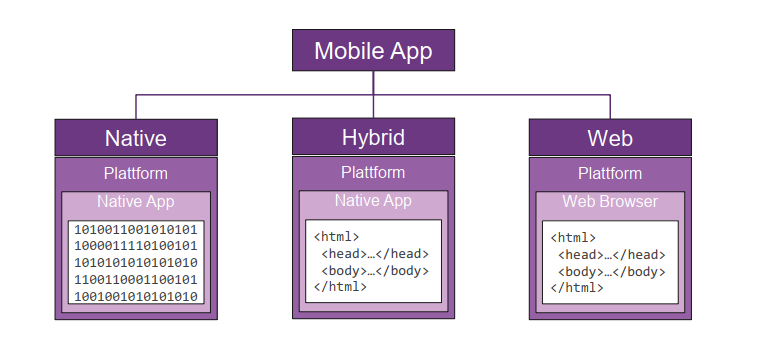
\includegraphics[scale=0.5]{Bilder/MobileApps.PNG}
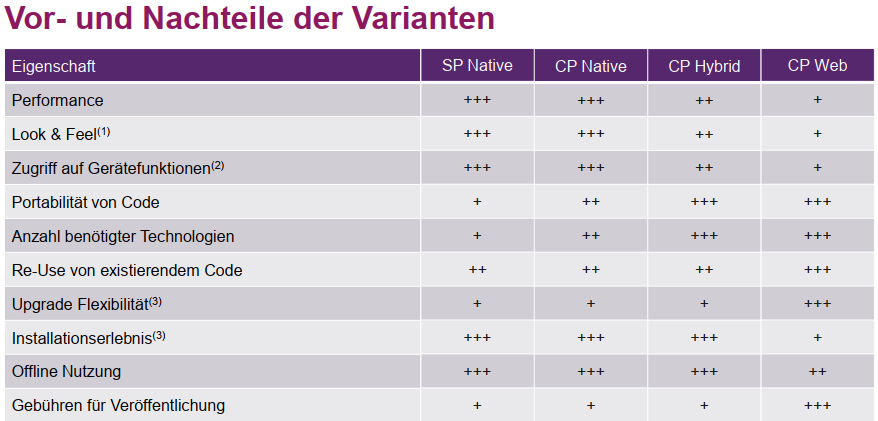
\includegraphics[scale=0.4]{Bilder/VorNachteileApps.PNG}
\section{Grundprinzipien}
Apps bestehen aus lose gekoppelten, wiederverwendbaren \textbf{Komponenten} (\textbf{Activities, Content Providers, Services und Broadcast Receivers}). Android hat die Kontrolle über ausgeführte Apps (\textbf{Verwaltung des Lebenszyklus, Kommunikation zwischen Komponenten, Terminierung bei Bedarf} (z.B. Speicherknappheit))



\section{Activities}
\begin{itemize}[leftmargin=*]
\item{Activities sind die Grundbausteine einer App}
\item{Eine Activity ~ eine Aufgabe ("Aktivität"), Kontakt suchen, Fotos anschauen}
\item{Jede App enthält 1-n Activities}
\item{Beim App-Start wird die Main Activity von Android erzeugt und ausgeführt}
\item{Registrierung im AndroidManifest.xml nötig}
\item{Activities besitzen eine grafische Oberfläche und verarbeiten Benutzereingaben}
\end{itemize}

\subsection{Activity Lifecycle}
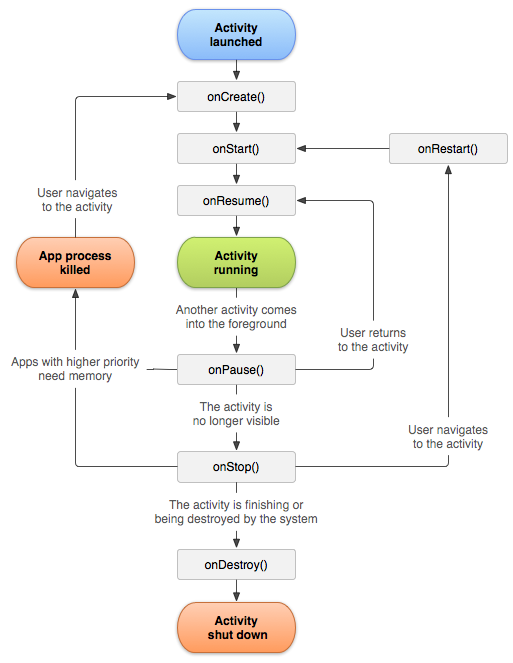
\includegraphics[scale=0.5]{Bilder/activity_lifecycle.png}

\subsubsection{Typische Anwendungsfälle}
\begin{itemize}[leftmargin=*]
\item{Erzeugung des GUI: onCreate()}
\item{Datensicherung: onPause() für schnelle Operationen, ansonsten onStop()}
\item{Dienste wie Lokalisierung aktivieren/deaktivieren: onResume() und onPause()}
\item{Zustand des GUI erhalten, z.B. bei Rotation: onSaveInstanceState() und onRestoreInstanceState()}
\end{itemize}

\section{Intents}
\begin{itemize}[leftmargin=*]
\item{Die Kommunikation zwischen Komponenten erfolgt über Intents (Absicht, Vorhaben)}
\item{Explizit: Aufruf einer definierten Komponente (typischerweise für Komponenten der eigenen App)}
\item{Implizit: Aufruf einer passenden Komponente (typischerweise für Komponenten aus anderen Apps)}
\item{Apps können sich im Android Manifest mit Intent Filters auf implizite Intents registrieren}
\item{Intents werden stets von Android verarbeitet}
\end{itemize}

\begin{minted}{Java}
--MainActivity.java--
// Expliziter Intent
Intent secondActivityIntent = new Intent(this,
SecondActivity.class);
startActivity(secondActivityIntent);
// Impliziter Intent
Intent sendIntent = new Intent();
sendIntent.setAction(Intent.ACTION_SEND);
sendIntent.setType("text/plain");
sendIntent.putExtra(Intent.EXTRA_TEXT, "Hey!");
startActivity(sendIntent);

--SecondActivity.java--
Intent intent = this.getIntent();
Bundle extras = intent.getExtras();
int parameter = extras.getInt("myKey");
SecondActivity.java
\end{minted}

Rückgabewert erhalten via Callback, non-blocking
\begin{minted}{Java}
startActivitiyForResult(intent, CODE);
@Override
protected void onActivityResult(int requestCode, int resultCode,
Intent data) { ... }
//Receiving End
this.setResult(Activity.Result_OK); this.finish();
\end{minted}

Prüfen ob Empfänger vorhanden (Muss nicht immer so sein, Exception)
\begin{minted}{Java}
boolean hasReceiver =
intent.resolveActivity(getPackageManager()) != null;
\end{minted}
AndroidManifest.xml
\begin{minted}{xml}
<uses-permission
android:name="android.permission.QUERY_ALL_PACKAGES" />
\end{minted}
\subsubsection{Back Stack}
Ausgeführte Activities werden im Back Stack verwaltet\\
Activities eines Stacks können zu verschiedenen Apps gehören\\
Dieselbe Activity kann mehrfach im selben Stack enthalten sein
\subsubsection{Tasks}
Ein Back Stack wird auch Task genannt\\
Android verwaltet die Ausführung von Tasks\\
Mittels Overview Screen kann zwischen Tasks gewechselt werden\\
Bei Bedarf können Activities in neuen Tasks gestartet werden
\subsection{Prozesse}
Jedes APK hat einen eigenen Linux User und einen eigenen Linux Prozess. Jeder Prozess hat mindestens einen Thread (MainThread). Das schützt vor gegenseitigen Speicherzugriffen
\subsubsection{Main Thread}
Achtung: nur der Main Thread darf das GUI
aktualisieren, sonst Exception\\
Option 1: Activity.runOnUiThread(Runnable)\\
Option 2: View.post(Runnable)\\
Option 3: Handler und Looper\\

\subsubsection{Event Handling im Code}
\begin{minted}{Java}
final TextView textView = this.findViewById(R.id.text_example);
Button button = this.findViewById(R.id.button_example);
button.setOnClickListener(v -> { 
    textView.setText("Button pressed"); 
});
\end{minted}
\subsubsection{Event Handling im XML}
Die Auflösung erfolgt zur Laufzeit via Reflection.\\
Code-Variante bevorzugen (Trennung von UI und Logik)
\begin{minted}{XML}
android:onClick="onExampleButtonClicked
\end{minted}
\subsubsection{Resources}
In Android werden alle Dateien, die keinen
Code enthalten, als Resources bezeichnet\\
Zugriff erfolgt über Resource IDs\\
Zugriff via R-Klasse

In XML können Resources mittels @-Notation abgerufen werden:
\\@\java{[<package_name>:]<resource_type>/<resource_name>}\\
Neue IDs für UI-Elemente werden mit @+id/ erzeugt

\subsubsection{Value-Resources}

\textcolor{red}{colors.xml} für Farbwerte \\
\textcolor{red}{dimens.xml} für Dimensionen\\
\textcolor{red}{strings.xml} für Texte\\
\textcolor{red}{styles.xml} für Styles\\

Bei Value-Resources enthält eine Datei mehrere Ressourcen\\
• Sonst gilt eine Datei = eine Ressource (z.B. Layouts)
Empfehlungen\\
• Veränderliche Werte immer in passenden Files definieren und referenzieren\\
• Gilt insbesondere für mehrfach verwendete Werte (z.B. Farben, Schriftgrössen, ...)\\

\subsection{Dimensionen}
\textbf{dp}: Density-independent Pixels\\
\textbf{sp}: Scale-independent Pixels\\
\textbf{px}: Pixel\\
\textbf{pt}: Punkte (1/72 eines physikalischen)\\
\textbf{in}: Inch\\
\textbf{mm}: Millimeter\\
\textbf{Empfehlungen}\\
- \textbf{Schriften immer} in \textbf{sp} \\
- \textbf{Alles andere} in \textbf{dp} \\

\subsection{Qualifier}
Die Auslagerung in XML-Dateien dient nicht nur der sauberen Trennung\\
Resources können in unterschiedlichen Varianten hinterlegt werden\\
• Texte für verschiedenen Sprachen\\
• Bilder für verschiedenen Auflösungen\\
• Layouts für unterschiedliche Gerätetypen\\
Zur Unterscheidung werden die Verzeichnisnamen mit Qualifiern ergänzt\\
• Liste der Qualifier\\
• Qualifier können kombiniert werden\\
• Reihenfolge der Qualifier muss korrekt sein\\
• Wizard in Android Studio hilft dabei\\
Android lädt automatisch die passendsten Ressourcen
\subsection{Assets}
Resources im res/-Ordner können nur via Resource ID zugegriffen werden\\
Ist der Zugriff auf die Originaldateien oder Dateistruktur nötig, so müssen diese Dateien im
assets/-Ordner platziert werden\\
Via AssetManager-Klasse kann dieser Ordner wie ein Dateisystem gelesen werden\\
Achtung: die Verwendung von Qualifiers ist nicht möglich
\subsection{App Manifest}
Das AndroidManifest.xml enthält essenzielle Informationen zur App
• ID, Name, Version und Logo\\
• Enthaltene Komponenten\\
• Hard- und Softwareanforderungen\\
• Benötigte Berechtigungen
\subsection{Application ID und Version}
\subsubsection{package}
• Eindeutige Identifikation der App\\
• Definiert den Namespace für die Anwendung\\
• Reversed Internet Domain-Format
\subsubsection{versionName}
• Ein menschenlesbarer String\\
• Typischerweise Semantic Versioning
\subsubsection{versionCode}
• Ein positiver Integer für interne Verwendung\\
• Je höher die Zahl, desto "neuer" die App\\
• Unterschiedliche Ansätze zur Inkrementierung

\subsection{Application-Element}
AndroidManifest.xml
\begin{minted}{XML}
<application android:name="MyApplication">
<!-- gekürzt -->
</application>
\end{minted}
• Application ist auch eine Klasse, die den
globalen Zustand unserer App hält, und enthält überschreibbare Lifecycle-Methoden\\
• Wir können optional eine eigene Ableitung
von Application registrieren\\

\section{Rückwärtskompatibilität}
\subsection{API Levels}
Das API Level ist eine Zahl, welche die Version der Android API identifiziert\\
Jedes Level enthält immer alle älteren APIs, ggf. aber deprecated\\
Um möglichst viele Geräte zu erreichen, sollte der API möglichst niedrig sein\\
Bestimmte Funktionen sind jedoch nur in neueren API Levels verfügbar\\
Android Studio unterstützt bei der Wahl des passenden Levels\\
\subsection{API Levels im Manifest und Gradle}
\textbf{minSdkVersion} gibt an, welche Version das
Gerät mindestens haben muss\\
\textbf{maxSdkVersion} gibt an, welche Version das
Gerät maximal haben darf
Android ignoriert diesen Wert seit Version 2.0.1
Der Google Play Store verwendet ihn als Filter\\
\textit{Empfehlung: nicht verwenden}\\
\textbf{targetSdkVersion} ist die höchste Version,
mit welcher die App getestet wurde\\
\textbf{compileSdkVersion} gibt an, mit welcher API
die App kompiliert wird\\
minSdkVersion <= targetSdkVersion <= compileSdkVersion

\subsection{Android Jetpack und AndroidX}
AndroidX ersetzt Android Support Libraries\\
• AppCompat(Library in Jetpack) macht neue Features auf tieferen API\\
Levels verfügbar\\
• Grundidee: Verwendung von Elementen aus
dem androidx-Namespace anstelle der
normalen Android-Komponenten


\section{GUI}
Das GUI kann auf zwei Arten erstellt werden\\
• Deklarativ: Beschreibung in XML\\
• Imperativ: Beschreibung im Quellcode

GUI-Elemente werden hierarchisch angeordnet\\
• View: Widgets (Controls)\\
• ViewGroup: Layouts (Container)\\

Die Basisklasse aller GUI-Elemente ist View\\
ViewGroup-Klassen werden auch Layouts(1) oder Container genannt

\section{Layouts}
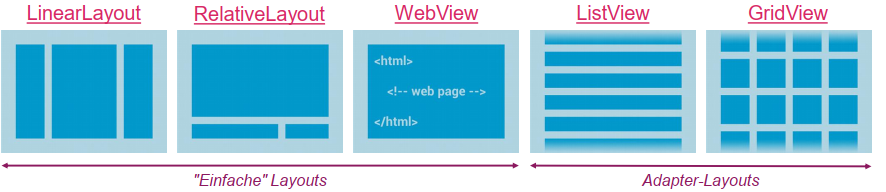
\includegraphics[scale=0.4]{Bilder/layouts.PNG}
Layouts können beliebig geschachtelt werden – mit negativem Einfluss auf die Performance\\
• Bevorzugt sind breite, flache Hierarchien\\
Auch sind die mit \xml{layout_}-Parametern definiert Werte nur Wünsche an das Eltern-Layout;
diese müssen beim Berechnen der realen Grössen ggf. ignoriert werden

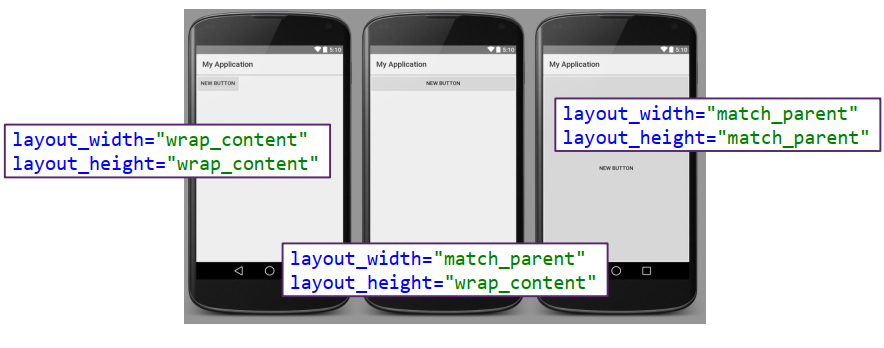
\includegraphics[scale=0.4]{Bilder/wrap_content-Match-parent.PNG}
\xml{layout_width}: Gewünschte Breite des Childs\\
\xml{layout_height}: Gewünscht Höhe des Childs
Zulässige Werte sind\\
• \xml{match_parent}: so gross wie möglich\\
("am liebsten so gross wie mein Parent-Layout")\\
• \xml{wrap_content}: so klein wie möglich\\
("nur gerade so gross, dass mein Inhalt Platz hat")\\
• Eine Zahl inkl. gültiger Dimension\\
(eher unüblich; wenn verwendet, dann mit dp)\\


\subsection{Linear Layout}
Durch Gewichte können die Grössen der Child-Elemente beeinflusst werden\\
• \xml{android:layout_weight="1"}\\
• Verwendung im Kombination mit \xml{"wrap_content"}\\
• Gewichte wirken immer in Richtung der "Orientierung"\\
• Kinder ohne Gewicht bekommen minimalen Platz, auf die restlichen Kinder wird die übrige\\ Fläche anteilsmässig entsprechend der Gewichte aufgeteilt\\

\begin{minted}{XML}
android:layout_margin="20dp" //Mit Layout
android:padding="20dp" //Ohne Layout
android:orientation="vertical
android:orientation="horizontal"
\end{minted}

\subsection{Frame Layout}
Kinder werden übereinander angeordnet \xml{android:translationZ}\\

\subsection{Relative Layout}
Kinder werden relativ zueinander angeordnet
\xml{android:layout_toEndOf}\\
Positions the start edge of this view to the end of the given anchor view ID.\\
\xml{android:layout_toLeftOf}\\
Positions the right edge of this view to the left of the given anchor view ID.\\
\xml{android:layout_toRightOf}\\
Positions the left edge of this view to the right of the given anchor view ID.\\
\xml{android:layout_toStartOf}\\
Positions the end edge of this view to the start of the given anchor view ID. 

\subsection{Constraint Layout}
Das modernste und flexibelste Layout in Android\\
• Teil von Android Jetpack / AndroidX\\
• Speziell für grosse, komplexe Layouts mit flacher Hierarchie entworfen\\
• Die Flexibilität bringt leider auch eine steile Lernkurve mit sich\\
Grundidee ist ähnlich zum Relative Layout\\
• Definieren von Beziehungen zwischen Views\\
• Pro View muss mindestens eine horizontale und eine vertikale Einschränkung definiert werden\\
Guter Support in Android Studio\\
\subsubsection{Animationen}
Verwendung der TransitionManager-Klasse\\
Zwei Layouts nötig: Start und Ende der Animation

\begin{minted}{Java}
private boolean displaysFirstLayout = true;
// innerhalb von onCreate()
setContentView(R.layout.activity_constraint);
TextView textViewA = findViewById(R.id.txtA);
ConstraintLayout constraintLayout = 
    findViewById(R.id.constraint_layout);
textViewA.setOnClickListener(v -> {
    int targetLayout = displaysFirstLayout ?
                        R.layout.activity_constraint_2 :
                        R.layout.activity_constraint;
    TransitionManager.beginDelayedTransition(constraintLayout);
    ConstraintSet constraintSet = new ConstraintSet();
    constraintSet.load(this, targetLayout);
    constraintSet.applyTo(constraintLayout);
    displaysFirstLayout = !displaysFirstLayout;
});
\end{minted}
% \definecolor{LightGray}{rgb}{0.90,0.90,0.90}
% \setminted[Java]{breaklines, bgcolor=LightGray}


\section{Widget (Controls)}
Ein Sammelbegriff für visuelle Elemente
des User Interfaces\\
Basisklasse ist View, nicht Widget

\begin{minted}{XML}
<TextView
android:text="TextView"
android:textSize="20sp"
android:textStyle="bold"
android:typeface="monospace"
android:textColor="@android:color/white"
android:background="@color/colorPrimaryDark"
android:drawableEnd="@drawable/ic_emoji"
android:drawableTint="@android:color/white"/>
<ImageView
android:layout_height="80dp"
android:src="@drawable/ic_emoji"
android:scaleType="fitCenter"
android:tint="@color/colorPrimaryDark" />
<Button
android:text="Button"
android:drawableEnd="@drawable/ic_emoji"
android:drawableTint="@color/colorPrimary"/>
<ImageButton
android:layout_height="30dp"
android:src="@drawable/ic_emoji"
android:scaleType="fitCenter"
android:tint="@color/colorPrimaryDark" />
\end{minted}
\subsubsection{<EditText />}
EditText dient als Eingabefeld für Texte und Zahlen\\
android:inputType beeinflusst Verhalten und aussehen\\
• Format (text, phone, date, textPassword, …)\\
• Korrekturoptionen (textAutoComplete, textAutoCorrect, …)\\
• Darstellung (textCapWords, textCapSentences, …)\\
• Mehrzeiligkeit (textMultiLine)\\
inputType-Werte sind kombinierbar, z.B.:\\
\xml{android:inputType="textCapCharacters|textAutoCorrect"}\\
Abhängig vom Typ wird passendes Keyboard angezeigt\\

Dazu muss eine Implementierung von TextWatcher als Listener registriert werden:\\
\java{myEditText.addTextChangedListener(new TextWatcher() { … })}

Das Interface umfasst 3 Methoden\\
• beforeTextChanged: wird aufgerufen, bevor der Text geändert wird
(wir sehen noch den alten Text)\\
• onTextChanged: wird aufgerufen, sobald der Text geändert hat
(meistens interessiert uns nur diese Methode)\\
• afterTextChanged: wird aufgerufen, nachdem der Text geändert wurde
(hier haben wir noch die Chance den Text anzupassen → Achtung vor Endlosschleife!)

Mit setError() wird eine Nachricht gesetzt,
bei jeder Änderung wird diese zurückgesetzt
\begin{minted}{Java}
EditText passwordInput = findViewById(R.id.edit_password);
passwordInput.addTextChangedListener(new TextWatcher() {
    // Methoden gekürzt
    @Override
    public void afterTextChanged(Editable editable) {
        if (editable.length() < 8) {
            passwordInput.setError("Passwort zu kurz.");
        }
    }
});
\end{minted}
\subsection{Toasts}
Einfache Rückmeldung zu einem Vorgang\\
• Darstellung in einem Popup-Fenster\\
• Keine Interaktion für Benutzer möglich\\
• Verschwinden nach kurzer Zeit automatisch
\begin{minted}{Java}
Context context = this;
String text = "MGE rocks!";
int duration = Toast.LENGTH_SHORT;
Toast toast = Toast.makeText(context, text, duration);
toast.show();
\end{minted}
\subsection{Snackbars}
Selber Einsatzzweck wie Toasts\\
Moderne Alternative für Toasts\\
Interaktionen mit Benutzer möglich
\begin{minted}{Java}
ViewGroup parent = findViewById(R.id.llSystemWidgets);
String text = "MGE rocks!";
int duration = Snackbar.LENGTH_LONG;
String action = "Schliessen";
Snackbar snackbar = Snackbar.make(parent,text, duration);
snackbar.setAction(action, v -> { snackbar.dismiss(); });
snackbar.show();
\end{minted}
\subsection{Dialoge}
Dialoge erzwingen eine Aktion vom Benutzer\\
Füllen Screen nicht vollständig\\
Viele Anpassungsmöglichkeiten
\begin{minted}{Java}
AlertDialog dialog;
dialog = new AlertDialog.Builder(this)
.setTitle("Beispiel")
.setMessage("Gutes Beispiel?")
.setCancelable(false)
.setPositiveButton("Ja", (d, id) -> { ... })
.setNegativeButton("Nein", (d, id) -> { ... })
.create();
dialog.show();
\end{minted}
\subsection{Notifications}
Nocitifcations(Mitteilung ausserhalb aktiver Nutzung, Darstellung an Statusbar / Notification Drawer / Heads-Up Notification / Lock Screen / App Icon Badge). NotificationCompat in AndroidX verwenden
\begin{minted}{Java}
// Konstanten und Variablen
final String CID = "MGE_Channel";
final String CNAME = "MGE Notifications";
final String CDESC = "Ein Channel für MGE ";
final int CIMP = NotificationManager.IMPORTANCE_HIGH;
int notificationId = 1;
// Manager aus AndroidX verwenden
NotificationManagerCompat manager;
manager = NotificationManagerCompat.from(this);
// Channel-Erzeugung ab Android 26
if (Build.VERSION.SDK_INT >= Build.VERSION_CODES.O) {
NotificationChannel channel;
channel = new NotificationChannel(CID, CNAME, CIMP);
channel.setDescription(CDESC);
manager.createNotificationChannel(channel);
}
// Notification erstellen und anzeigen
Notification notification;
notification = new NotificationCompat.Builder(this, CID)
.setSmallIcon(R.drawable.ic_emoji)
.setContentTitle("MGE")
.setContentText("MGE rocks!")
.build();
manager.notify(notificationId++, notification);
\end{minted}
\subsection{Menus}
API wurde schon oft erweitert\\
Menu wird als Resource in res/menu definiert
\begin{minted}{XML}
<?xml version="1.0" encoding="utf-8"?>
<menu xmlns:app="http://schemas.android.com/apk/res-auto"
xmlns:android="http://schemas.android.com/apk/res/android">
    <item android:id="@+id/menu_1"
    android:title="Menu 1"
    android:icon="@drawable/ic_bulb"
    app:showAsAction="always"/>
    ...
</menu>
\end{minted}
\begin{minted}{Java}
@Override
public boolean onCreateOptionsMenu(Menu menu) {
    MenuInflater inflater = getMenuInflater();
    inflater.inflate(R.menu.menu_example, menu);
    return true;
}
@Override
public boolean onOptionsItemSelected(MenuItem item) {
    switch (item.getItemId()) {
        case R.id.menu_1:
        break;
        ...
    }
    return true;
}
\end{minted}
\subsection{ScrollView}
• Die ScrollView ist ein spezielles Layout mit nur einem Kind-Element\\
• Es ergänzt eine Scrollbar und erlaubt das vertikale Scrolling des Inhaltes\\
• Horizontal Scrolling ist nur mit HorizontalScrollView möglich\\
• Alternative in AndroidX: NestedScrollView erlaubt beide Richtungen
\begin{minted}{XML}
<ScrollView
    android:layout_width="match_parent"
    android:layout_height="match_parent">
    <!-- Genau ein Kind hier -->
</ScrollView>
\end{minted}
\subsection{Collections}
Ein Adapter vermittelt zwischen Darstellung und Datenquelle (Adapter-Pattern)\\
Dadurch bleibt unser Datenmodell frei von UI-Logik (gutes Software Engineering)
\subsection{ListView und ArrayAdapter}
\begin{minted}{XML}
<?xml version="1.0" encoding="utf-8"?>
<ListView xmlns:android="…"
    android:id="@+id/list_example"
    android:layout_width="match_parent"
    android:layout_height="match_parent">
</ListView>
\end{minted}
\begin{minted}{Java}
setContentView(R.layout.activity_main);
String[] data = new String[] { ... };
ArrayAdapter<String> adapter = new ArrayAdapter<>(
        this, android.R.layout.simple_list_item_1,
        android.R.id.text1, data);
ListView listView = findViewById(R.id.list_example);
listView.setAdapter(adapter);
\end{minted}
\subsubsection{Ein eigener ArrayAdapter}
\begin{minted}{Java}
setContentView(R.layout.activity_main);
ArrayList<User> data = UserManager.getUsers();
UsersAdapter adapter = new UsersAdapter(this, data);
ListView listView = findViewById(R.id.list_example);
listView.setAdapter(adapter);

public class User {
    public String name;
    public int age;
    public User(String name, int age) {
        this.name = name;
        this.age = age;
    }
}
public class UsersAdapter extends ArrayAdapter<User> {
    public UsersAdapter(ctx c, ArrayList<User> users) {
        super(ctx, 0, users);
    }
    @Override
    public View getView(int pos, View view, ViewGroup parent) {
        if (view == null) {
            Context context = getContext();
            LayoutInflater inflater = LayoutInflater.from(context);
            view = inflater.inflate(
                android.R.layout.simple_list_item_2,
                parent, false);
        }
        TextView text1 = view.findViewById(android.R.id.text1);
        TextView text2 = view.findViewById(android.R.id.text2);
        User user = getItem(pos);
        text1.setText(user.name);
        text2.setText(user.age + " Jahre");
        return view;
    }
}
\end{minted}
\subsection{Viewholder}
Es gibt noch zwei weitere, teure Operationen in unserem Beispiel
\begin{minted}{Java}
    TextView text1 = view.findViewById(android.R.id.text1);
    TextView text2 = view.findViewById(android.R.id.text2);
\end{minted}
Effizienter wäre es, diese Objekt-Referenzen pro erzeugter View zu speichern\\
Genau dies ist die Idee hinter dem View Holder-Pattern
\begin{minted}{Java}
if (view == null) {
    //Inflate wie vorher
    viewHolder = new ViewHolder();
    viewHolder.text1 = view.findViewById(android.R.id.text1);
    viewHolder.text2 = view.findViewById(android.R.id.text2);
    view.setTag(viewHolder);
} else {
    viewHolder = (ViewHolder)convertView.getTag();
}
\end{minted}

\subsection{RecyclerView}
Die RecyclerView ist eine moderne Alternative zu ListView und GridView\\
• Integriertes View-Recycling\\
• Erzwungene Verwendung von View Holdern\\
• Weniger Overhead im eigenen Code\\
• Layout-Flexibilität durch LayoutManager\\
• Sie ist, ihr ahnt es schon, Teil von AndroidX\\
• Die Verwendung wird von Google empfohlen
\begin{minted}{XML}
<androidx.recyclerview.widget.RecyclerView
    android:id="@+id/recycler_view"
    android:layout_width="match_parent"
    android:layout_height="match_parent">
</androidx.recyclerview.widget.RecyclerView>
\end{minted}
\begin{minted}{Java}
    //MainActivity
    setContentView(R.layout.activity_recyclerview);
    RecyclerView recyclerView = findViewById(R.id.recycler_view);
    RecyclerView.LayoutManager layoutManager;
    layoutManager = new LinearLayoutManager(this);
    recyclerView.setLayoutManager(layoutManager);
    ArrayList<User> data = UserManager.getUsers();
    UsersAdapter adapter = new UsersAdapter(data);
    recyclerView.setAdapter(adapter);

public class UsersAdapter extends RecyclerView.Adapter<ViewHolder>{
    private ArrayList<User> users;
    @Override
    public ViewHolder onCreateViewHolder(ViewGroup parent, int vt) {
        Context context = parent.getContext();
        LayoutInflater inflater = LayoutInflater.from(context);
        View view = inflater.inflate(android.R.layout.simple_list_item_2,
        parent,false);
        return new ViewHolder(view,
            view.findViewById(android.R.id.text1),
            view.findViewById(android.R.id.text2)
        );
    }
    @Override
    public void onBindViewHolder(ViewHolder holder, int position) {
        User user = this.users.get(position);
        holder.text1.setText(user.name);
        holder.text2.setText(user.age + " Jahre");
    }
    @Override
    public int getItemCount() {
        return this.users.size();
    }
}

private class ViewHolder {
    TextView text1;
    TextView text2;
}
\end{minted}
\section{Fragments}
Activities können nicht kombiniert werden – dafür aber Fragments
Zusätzliche Callbacks gegenüber Activity\\
• onAttach: Fragment an Activity angehängt\\
• onCreateView: UI des Fragments erstellen\\
• onActivityCreated: Activity wurde erzeugt\\
• onDestroyView: Gegenstück zu onCreateView\\
• onDetach: Gegenstück zu onAttach\\
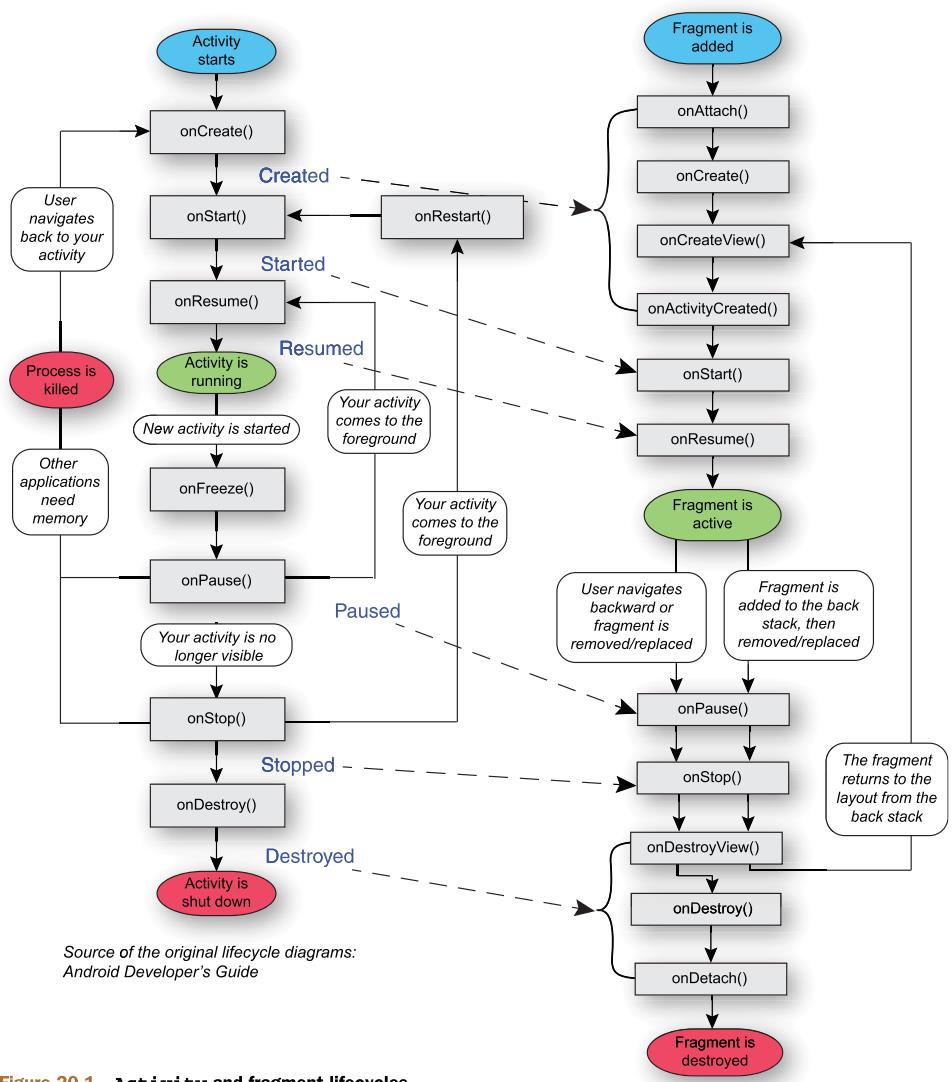
\includegraphics[scale=0.35]{Bilder/fragments_lifecycle.png}
\subsection{Statische Einbindung}
\begin{minted}{XML}
<fragment android:name="(…).OutputFragment"
android:id="@+id/main_fragment_output"
android:layout_width="match_parent"
android:layout_height="match_parent" />
\end{minted}
\begin{minted}{Java}
public class OutputFragment extends Fragment {
    @Override
    public View onCreateView(LayoutInflater inflater,
    ViewGroup container, Bundle savedInstanceState) {
        return inflater.inflate(R.layout.fragment_output,
        container, false);
    }
}
\end{minted}
\subsection{Dynamische Einbindung}
Vorteil: Austauschbarkeit, keine direkten Abhängigkeiten zu Activities
\begin{minted}{XML}
<LinearLayout xmlns:android="(…)"
android:layout_width="match_parent"
android:layout_height="match_parent">
    <FrameLayout android:id="@+id/main_fragment_container"
    android:layout_width="match_parent"
    android:layout_height="match_parent" />
</LinearLayout>
\end{minted}
\begin{minted}{Java}
FragmentManager mgr = getSupportFragmentManager();
FragmentTransaction trans = mgr.beginTransaction();
OutputFragment fragment = new OutputFragment();
trans.add(R.id.main_fragment_container, fragment);
trans.commit();
\end{minted}
\subsection{Kommunikation}
\textbf{Parameter \& Methoden}: Activity -> Fragment\\
\textbf{Callback}: Activity <- Fragment
\begin{minted}{Java}
fragment = OutputFragment.create("Initial Value");
...
button.setOnClickListener(v -> {
    fragment.updateText("Updated value");});

public class OutputFragment extends Fragment {
    private TextView textOutput;
    public static OutputFragment create(String text) {
        Bundle args = new Bundle();
        args.putString("Key", text);
        OutputFragment fragment = new OutputFragment();
        fragment.setArguments(args);
        return fragment;
    }
    @Override
    public View onCreateView(...) {
        View fragment = inflater.inflate(...);
        textOutput = fragment.findViewById(R.id.output_text);
        String param = getArguments().getString("Key");
        updateText(param);
        return fragment;
    }
    public void updateText(String text) {
        textOutput.setText(text);
    }
}
\end{minted}

\subsection{Callback Interfaces}
\begin{minted}{Java}
public class MainActivity extends AppCompatActivity
implements OutputFragmentCallback {
...
public interface OutputFragmentCallback {
    void onTextTapped(String text);
}
...
public class OutputFragment extends Fragment {
    private OutputFragmentCallback callback;
    @Override
    public void onAttach(Context context) {
        super.onAttach(context);
        try {
            callback = (OutputFragmentCallback) context;
        } catch (ClassCastException e) {
            throw new ClassCastException("...");
        }
    }
    @Override
    public View onCreateView(...) {
        View fragment = inflater.inflate(...);
        textOutput = fragment.findViewById(R.id.output_text);
        textOutput.setOnClickListener(v -> {
            callback.onTextTapped("…");
        });
        return fragment;
    }
}
\end{minted}

\subsection{Fragmente verschachteln}
Unterschied: \java{getChildFragmentManager()} anstelle von \java{getSupportFragmentManager()}

\subsection{Wann sind Fragments sinnvoll?}
Eintrittspunkt -> zwingend Activity

\section{Styling}
Widgets können im XML gestylt werden. Führt aber zu Code-Duplizierung, Inkonsistenzen und Unübersichtlichkeit.
Mit Styles können wir Formatierungen
wiederverwendbar machen
\begin{minted}{XML}
<style name="HeaderText.Big">
    <item name="android:textSize">40sp</item>
</style>
\end{minted}
\subsection{Theme}
Themes sind spezielle Styles, die für eine
ganze App oder einzelne Activities gelten
\begin{minted}{XML}
<style name="AppTheme" parent="…">
    <item name="android:textViewStyle">@style/MyText</item>
</style>
<style name="MyText">
    <item name="android:textSize">24sp</item>
    ...
</style>
\end{minted}
\subsubsection{Variante 1: Manifest}
\begin{itemize}[leftmargin=*]
\item{Für die ganze App (application)}
\item{Für einzelne Activities (activity)}
\end{itemize}
\begin{minted}{XML}
<application ... android:theme="@style/AppTheme">
    <activity ... android:theme="@style/AnotherAppTheme" />
</application>
\end{minted}
\subsubsection{Variante 2: Activity-Code}
\begin{itemize}[leftmargin=*]
\item{Innerhalb von onCreate()}
\item{Wichtig: vor setContentView()}
\end{itemize}
\begin{minted}{Java}
@Override
protected void onCreate(Bundle savedInstanceState) {
    setTheme(R.style.AnotherAppTheme);
    setContentView(R.layout.activity_styling);
}
\end{minted}
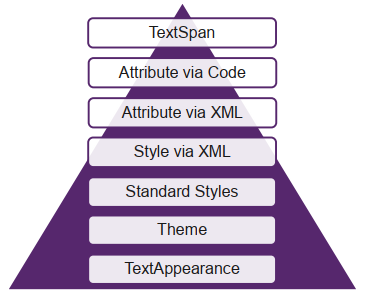
\includegraphics[scale=0.5]{Bilder/styleshirachie.PNG}
\subsection{Material}
Eine Design Language ist eine Hilfestellung für den Designprozess. Beschreibt wie Teile aussehen und sich verhalten. Ziel ist ein systemweites, konsistentes und benutzbares Look and Feel.\\
Material Design ist eine Design Language von Google mit physikalischem Material als Vorbild. Oberflächen erinnern an Papier und Tinte. Materialen reflektieren und werfen Schatten. Basiert auf Print-Medien. Bewegungen bedeuten Aktionen.\\
Material ist immer 1dp dick. Material hat eine unendliche Auflösung. Material kann sich verändern und bewegen. Die Flughöhe definiert, welches Element welche überlagert.\\
8dp-Raster
\begin{minted}{XML}
<style name="AppTheme" parent="...">
    <item name="colorPrimary">...</item>
    <item name="colorPrimaryDark">...</item>
    <item name="colorAccent">...</item>
</style>
\end{minted}
\subsection{Styles für Texte}
\xml{style="@style/TextAppearance.MaterialComponents.Headline3"/>}

---
\section{Berechtigung}
• Apps dürfen nur Aktionen ausführen, die andere Dienste
nicht negativ beeinflussen (Sandbox)\\
• Vor riskante Operationen müssen Berechtigungen eingeholt werden\\
Es gibt zwei Arten von Berechtigungen:\\
\textbf{Normal}: werden durch das System erteilt\\
\textbf{Gefährlich}: werden durch den Benutzer erteilt\\

Zugriff auf System APIs: Internet, WiFi, Bluetooth\\
Zugriff auf sensitive Daten: Telefonbuch, Kalender\\
Zugriff auf Hardware: Kamera, Lokalisierung\\

Empfehlung: vor jedem Zugriff auf geschützte APIs Status überprüfen\\
Andernfalls droht SecurityException

Best Practices
\begin{itemize}[leftmargin=*]
\item{Nur anfordern, was auch benötigt wird}
\item{Im Kontext der Verwendung anfordern}
\item{Transparente Erklärungen}
\item{Abbruch ermöglichen}
\item{Verweigerung berücksichtigen}
\end{itemize}

\subsubsection{Manifest}
Benötigte Berechtigungen müssen im
Manifest deklariert werden
\begin{itemize}[leftmargin=*]
\item{Knoten <uses-permission}
\item{Obergrenze für API-Level definierbar}
\end{itemize}

Hinweise auf benötigte Features für Filterung im Google Play Store
\begin{itemize}[leftmargin=*]
\item{Knoten \xml{<uses-feature>}}
\item{Optional, aber empfohlen}
\item{required="true" → notwendig (Standard)}
\end{itemize}
\begin{minted}{Java}
private static final int CALLBACK_CODE = 1;
String permission = Manifest.permission.CALL_PHONE;
// Aktuellen Status prüfen (AndroidX)
int status = ContextCompat.checkSelfPermission(this, permission);
if (status != PackageManager.PERMISSION_GRANTED) {
    if (shouldShowRequestPermissionRationale(permission)) {
    // Erklärung für Benutzer anzeigen (Wozu nötig?)
    }
    // Berechtigung beim Benutzer anfordern
    requestPermissions(
    new String[]{ permission },
    CALLBACK_CODE);
}
\end{minted}

\begin{minted}{Java}
@Override
public void onRequestPermissionsResult(
int requestCode, String[] permissions, int[] results) {
    if (requestCode != CALLBACK_CODE)
        return;
    if (results.length == 0)
        return; // Anfrage abgebrochen
    if (results[0] == PackageManager.PERMISSION_GRANTED) {
        // Berechtigung erteilt
    } else {
        // Berechtigung verweigert
    }
}
\end{minted}

\section{Persistenz}
\subsubsection{Speicherarten}
\textbf{Interner Speicher}
\begin{itemize}[leftmargin=*]
\item{Stets verfügbar}
\item{Geschützter Speicherbereich pro App}
\item{Speicherplatz begrenzt}
\item{Für app-interne Daten}
\end{itemize}
\textbf{Externer Speicher}
\begin{itemize}[leftmargin=*]
\item{Nicht immer verfügbar}
\item{Oft ein Wechseldatenträger}
\item{Emulation durch Android möglich}
\item{Speicherplatz begrenzt (aber meist grösser)}
\item{Primär für geteilte Daten}
\end{itemize}

\subsubsection{App-spezifische Dateien}
\begin{itemize}[leftmargin=*]
\item{Eigene, proprietäre Datenformate}
\item{Interner oder externer Speicher}
\item{Bei Deinstallation der App gelöscht}
\item{Geschützt vor fremdem Zugriff}
\end{itemize}

\begin{minted}{Java}
// Schreiben
File folder = getFilesDir();
File file = new File(folder, "my_file.txt");
String input = "MGE Beispiel";
FileOutputStream outputStream = new FileOutputStream(file);
outputStream.write(input.getBytes());
outputStream.close();
// Dateien anzeigen
for(File fileInFolder : folder.listFiles()) {
    Log.d("MGE.V05", "File: " + fileInFolder.getName());
}
// Lesen
int length = (int) file.length();
byte[] bytes = new byte[length];
FileInputStream inputStream = new FileInputStream(file);
inputStream.read(bytes);
inputStream.close();
String output = new String(bytes);
\end{minted}
\subsubsection{Preferences}
\begin{itemize}[leftmargin=*]
\item{Key-Value-Paare}
\item{Interner Speicher}
\item{Bei Deinstallation der App gelöscht}
\item{Keine Berechtigungen nötig}
\item{Zugriff via SharedPreferences-Objekte}
\end{itemize}

\begin{minted}{Java}
String file = "ch.ost.rj.mge.v05.myapplication.preferences";
String key1 = "my.key.1";
String key2 = "my.key.2";
String key3 = "my.key.3";
int mode = Context.MODE_PRIVATE;
// Objekt abholen
SharedPreferences preferences;
preferences = getSharedPreferences(file, mode);
// Schreiben
SharedPreferences.Editor editor = preferences.edit();
editor.putString(key1, "MGE Beispiel");
editor.putBoolean(key2, true);
editor.putInt(key3, 42);
editor.commit();
// Lesen
String value1 = preferences.getString(key1, "default");
boolean value2 = preferences.getBoolean(key2, false);
int value3 = preferences.getBoolean(key3, 0);
\end{minted}
\subsubsection{Content Providers}
Datenquellen für andere Apps(Kalender, Kontakte, Medien, etc.)\\
Client-Server Modell\\
Client: Content Resolver\\
Server: Content Provider\\
\subsubsection{Content Resolvers}
\begin{minted}{Java}
Cursor cursor = getContentResolver().query(uri, projection,
selection, selectionArgs, sortOrder);
\end{minted}
\subsection{Medien}
• Teilbare Bilder, Videos und Musik\\
• Externer Speicher\\
• Bleiben bei Deinstallation der App erhalten\\
• Zugriff via MediaStore (Content Provider), Berechtigung nötig

\subsection{Dokumente}
• Teilbare Dokumente wie PDF, ZIP, etc
• Externer Speicher\\
• Bleiben bei Deinstallation der App erhalten\\
• Zugriff via Storage Access Framework\\
• Auswahl von Dokumenten via "Picker", keine Berechtigung nötig

\begin{minted}{Java}
private static final int CREATE_DOCUMENT_CODE = 1;
private static final int OPEN_DOCUMENT_CODE = 2;
private static final String FILE_NAME = "my_file.txt";
private static final String FILE_TYPE = "text/plain";
// Intent zum Schreiben eines Dokuments
Intent intent = new Intent(Intent.ACTION_CREATE_DOCUMENT);
intent.addCategory(Intent.CATEGORY_OPENABLE);
intent.setType(FILE_TYPE);
intent.putExtra(Intent.EXTRA_TITLE, FILE_NAME);
startActivityForResult(intent, CREATE_DOCUMENT_CODE);
// Intent zum Öffnen eines Dokuments
Intent intent = new Intent(Intent.ACTION_OPEN_DOCUMENT);
intent.addCategory(Intent.CATEGORY_OPENABLE);
intent.setType(FILE_TYPE);
startActivityForResult(intent, OPEN_DOCUMENT_CODE);

@Override
public void onActivityResult(int req, int res, Intent data) {
    super.onActivityResult(req, res, data);
    switch(req) {
        case CREATE_DOCUMENT_CODE:
            if (res == Activity.RESULT_OK) {
                Uri uri = data.getData();
                // Mit Content Resolver Uri verarbeiten
            }
            break;
        case OPEN_DOCUMENT_CODE:
            if (res == Activity.RESULT_OK) {
                Uri uri = data.getData();
                // Mit Content Resolver Uri verarbeiten
            }
    }
}
\end{minted}
\subsection{Datenbanken}
• Strukturierte Daten\\
• Interner Speicher\\
• Bei Deinstallation der App gelöscht\\
• Keine Berechtigungen nötig\\
• Zugriff via SQLite API oder Room aus AndroidX / Jetpack
\subsubsection{Datenbanken – Room}
\begin{itemize}[leftmargin=*]
\item{ORM (Object Relational Mapping)}
\item{Weniger Code nötig (z.B. Mapping)}
\item{Überprüfung von Queries zur Compile-Zeit}
\item{Kompatibilität mit Jetpack-Komponenten}
\end{itemize}

\begin{minted}{Java}
@Entity
public class Entry {
    @PrimaryKey(autoGenerate = true)
    public int id;
    @ColumnInfo
    public String content;
}

@Dao
public interface EntryDao {
    @Query("SELECT * FROM entry")
    List<Entry> getEntries();
    @Insert
    void insert(Entry entry);
    @Delete
    void delete(Entry entry);
}

@Dao
public interface EntryDao {
    @Query("SELECT * FROM entry")
    List<Entry> getEntries();
    @Insert
    void insert(Entry entry);
    @Delete
    void delete(Entry entry);
} 

// Erzeugung DB-Objekt (MainActivity.java)
EntryDatabase db = Room.databaseBuilder(
this, EntryDatabase.class, "room.db").build();
EntryDao dao = db.entryDao();
// Daten einfügen
Entry entry = new Entry();
entry.content = "MGE Vorlesung";
dao.insert(entry);
// Daten auslesen
List<Entry> entries = dao.getEntries();
for (Entry entry : entries) {
    Log.d(null, + entry.id + " | " + entry.content);
}
// Aufräumen
db.close();

\end{minted}

\subsection{Debugging}
• Device File Explorer in Android Studio

\section{Hardwarezugriff}

\subsection{Sensor Framework}
• Framework für verschiedene Sensoren
\begin{itemize}[leftmargin=*]
\item{\java{SensorManager} als Einstiegspunkt}
\item{\java{Sensor} als Repräsentant für realen Sensor}
\item{\java{SensorEvent} enthält Werte des Sensors}
\item{\java{SensorEventListener} für Callbacks}
\end{itemize}

Verzögerung beeinflusst Energieverbrauch
• \java{SENSOR_DELAY_FASTEST} (0ms)\\
• \java{SENSOR_DELAY_GAME} (20ms)\\
• \java{SENSOR_DELAY_UI} (60ms)\\
• \java{SENSOR_DELAY_NORMAL} (200ms)

Änderung der Genauigkeit\\
• \java{SENSOR_STATUS_ACCURACY_HIGH}\\
• \java{SENSOR_STATUS_ACCURACY_MEDIUM}\\
• \java{SENSOR_STATUS_ACCURACY_LOW}\\
• \java{SENSOR_STATUS_ACCURACY_UNRELIABLE}\\
\begin{minted}{Java}
// Bei Sensor für Änderungen registrieren
String service = Context.SENSOR_SERVICE;
int type = Sensor.TYPE_LIGHT;
int delay = SensorManager.SENSOR_DELAY_NORMAL;
SensorManager mgr = (SensorManager)getSystemService(service);
Sensor sensor = mgr.getDefaultSensor(type);
mgr.registerListener(this, sensor, delay);
// Implementierung von SensorEventListener
@Override
public void onSensorChanged(SensorEvent sensorEvent) {
float lux = sensorEvent.values[0];
    Log.d(null, lux + " lux");
}
@Override
public void onAccuracyChanged(Sensor sensor, int i) { }

\end{minted}
Vibration -> 
Verwendung der Klasse Vibrator ->
Berechtigung nötig (VIBRATE). Sensor-Listener sollten in onPause() und onResume() abgemeldet/angemeldet werden
\begin{minted}{Java}
String service = Context.VIBRATOR_SERVICE;
int maxAmplitude = 255;
Vibrator vibrator = (Vibrator) getSystemService(service);
// Ab API 1
vibrator.vibrate(500);
Vibrator.cancel();
// Ab API 26
long[] durs = new long[]{ 500, 500, 500, 500, 500 };
int[] amps = new int[]{ 50, 100, 150, 200, 255 };
VibrationEffect effect;
effect = VibrationEffect.createOneShot(500, 255);
effect = VibrationEffect.createWaveform(durs, amps, -1);
vibrator.vibrate(effect);
// Ab API 29
int effectId = VibrationEffect.EFFECT_DOUBLE_CLICK;
effect = VibrationEffect.createPredefined(effectId);
vibrator.vibrate(effect);
\end{minted}
\subsubsection{Status der Internet-Verbindung}
Klasse ConnectivityManager\\
Üblich sind zwei Kanäle (Mobile \& Wifi)\\
• Android nutzt automatisch den besten Kanal\\
• Höhere Geschwindigkeit\\
• Bessere Signalqualität\\
• Kein Roaming
Needs \java{ACCESS_NETWORK_STATE}
\begin{minted}{Java}
String service = Context.CONNECTIVITY_SERVICE;
ConnectivityManager manager;
manager = (ConnectivityManager) getSystemService(service);
// Aktive Verbindung prüfen
NetworkInfo activeNetwork = manager.getActiveNetworkInfo();
if (activeNetwork != null) {
    int type = activeNetwork.getType();
    Log.d(null, "Active connection: " + type);
}
// Verbindungen prüfen
for (Network network : manager.getAllNetworks()) {
    NetworkInfo info = manager.getNetworkInfo(network);
    boolean state = info.isConnected();
    if (info.getType() == ConnectivityManager.TYPE_WIFI) {
        Log.d(null, "WiFi is connected: " + state);
    }
    if (info.getType() == ConnectivityManager.TYPE_MOBILE) {
        Log.d(null, "Mobile is connected: " + state);
    }
}
\end{minted}

\subsubsection{Kamera}
\begin{itemize}[leftmargin=*]
\item{Option 1: Apps via Intents starten}
\item{Option 2: Camera-API}
\item{Option 3: camera2-API}
\item{Option 4: CameraX-API (AndroidX)}
\end{itemize}
Vorteile von Option 1:
\begin{itemize}[leftmargin=*]
\item{Keine Berechtigungen nötig}
\item{Weniger Logik und Komplexität}
\end{itemize}
Vorteile von Optionen 2 bis 4
\begin{itemize}[leftmargin=*]
\item{Kamera Teil der eigenen App}
\item{Mehr Möglichkeiten und Kontroll}
\end{itemize}
\section{Architektur}
\begin{itemize}[leftmargin=*]
\item{Presentation}
\begin{itemize}[leftmargin=*]
\item{Darstellung und Interaktion mit Benutzer}
\item{Typischerweise stark an UI-Toolkit gebunden}
\item{Zugriff auf Domain-Schicht}
\end{itemize}
\item{Domain}
\begin{itemize}[leftmargin=*]
\item{Businesslogik und Domänenklassen}
\item{Keine UI-Funktionalität}
\item{Wenig externe Abhängigkeiten}
\item{Einfach zu testen}
\end{itemize}
\item{Data}
\begin{itemize}[leftmargin=*]
\item{Speicherung der Daten}
\item{Stellt Daten der Domain zur Verfügung}
\item{Auch Persistenz oder Datenhaltung genannt}
\end{itemize}
\end{itemize}
Observer Pattern\\
• Zwei Rollen\\
• Subject (wird beobachtet, z.B. Model-Klasse)\\
• Observer (beobachtet, z.B. View-Klasse)\\

Model-View-Controller
\begin{itemize}[leftmargin=*]
\item{\textcolor{red}{Model} beinhaltet die Daten (Java-Klassen)}
\item{\textcolor{red}{View} liest die Daten des Modells und zeigt diese an (View, Adapter)}
\item{\textcolor{red}{Controller} erhält Events der View und manipuliert das Model (Activity, Fragment)}

\subsection{Application}
\begin{itemize}[leftmargin=*]
\item{Der Eltern-Knoten unserer Komponenten im
Manifest heisst \textcolor{red}{application}}
\item{Zu diesem Knoten wird beim Start eine
Instanz der \textcolor{red}{Application}-Klasse erzeugt}
\item{Eigene Ableitungen der Klasse sind möglich}
\begin{itemize}[leftmargin=*]
\item{Einmalige Initialisierungen}
\item{Erzeugung von Singleton-Objekten}
\item{Zugriff auf globale Objekte}
\end{itemize}
\item{\textcolor{red}{Lifecycle-Methoden} werden von Android zu
bestimmten Zeitpunkten aufgerufen}
\end{itemize}
\end{itemize}


\begin{itemize}[leftmargin=*]
\item{onCreate()}
\begin{itemize}[leftmargin=*]
\item{Einmalig nach dem Start der App}
\item{Vor Erzeugung anderer App-Komponenten}
\end{itemize}
\item{onTerminate()}
\begin{itemize}[leftmargin=*]
\item{Wird auf realen Geräten nie aufgerufen}
\item{Reminder: Apps können stets beendet werden}
\end{itemize}
\item{onConfigurationChanged(newConfig)}
\begin{itemize}[leftmargin=*]
\item{Bei Änderungen der System-Konfiguration}
\item{Parameter enthält neue Konfiguration}
\item{Beispiel: Rotation des Gerätes}
\end{itemize}
\item{onLowMemory()}
\begin{itemize}[leftmargin=*]
\item{Bei Speicherknappheit des Systems}
\item{Hinweis auf mögliche Terminierung der App}
\end{itemize}
\item{onTrimMemory(level)}
\begin{itemize}[leftmargin=*]
\item{Bei geeigneten Momenten für Aufräumaktionen}
\item{Parameter gibt Hinweise auf Auslöser}
\item{Beispiel: App geht in den Hintergrund \java{(TRIM_MEMORY_UI_HIDDEN)}}
\end{itemize}
\end{itemize}

Via Application-Klasse kann der Lebenszyklus aller Activities überwacht werden

\subsubsection{Context}
Context ist eine abstrakte Klasse der SDK
mit über 50 Ableitungen (!), beispielsweise\\
• Activity\\
• Application
\begin{itemize}[leftmargin=*]
\item{Context-Objekte haben eine eingeschränkte Lebensdauer}
\begin{itemize}[leftmargin=*]
\item{Angeforderte Ressourcen werden mit dem zugehörigen Context freigegeben}
\item{Beispiel: Activity-Context via this}
\end{itemize}
\item{Das Application Context-Objekt ist während der ganzen App-Lebensdauer gültig}
\begin{itemize}[leftmargin=*]
\item{Abholen via Context.getApplicationContext()}
\item{Eingeschränkt verwendbar für UI-Aktionen}
\item{Vorsicht vor Memory Leaks}
\end{itemize}
\end{itemize}

\subsection{Broadcasts}
Austausch von Meldungen zwischen Apps
Zwei Arten von Broadcasts:\\
• \textbf{Lokal}: innerhalb einer App
• \textbf{Global}: innerhalb des ganzen Systems

\textbf{Broadcasts empfangen}\\
\textbf{Statische Registrierung} im Manifest vs. \textbf{Dynamische Registrierung} via Context. 
Implizite Broadcasts können nur von dynamischen Registrierungen empfangen werden, wegen einer Änderung im API 26. Explizite Broadcasts können via statische und dynamische Registrierung emfpangen werden.\\
\textbf{Broadcasts versenden}
\begin{itemize}[leftmargin=*]
\item{Broadcasts sind normale Intent-Objekte}
\item{Die Action im Intent definiert den Ereignistyp}
\item{Parameter sind als Extras möglich}
\end{itemize}
\textit{Für lokale Nachrichten immer LocalBroadcastManager verwenden}
\subsubsection{Best Practices}
\begin{itemize}[leftmargin=*]
\item{Dynamische Registrierung bevorzugen}
\item{Lokale Broadcasts bevorzugen}
\item{Keine sensitiven Daten in Broadcasts übermitteln}
\item{App ID in eigene Broadcast-Actions integrieren}
\item{Schnelle Rückkehr aus onReceive()}
\item{Falls App nicht aktiv: keine Activity starten}
\end{itemize}
\subsection{Services}
Ab API 30 werden die normalen Java-Klassen für Background Threads empfohlen\\
\begin{itemize}[leftmargin=*]
\item{Ausführung von Aktionen im Hintergrund}
\item{Lebenszyklus unabhängig von App}
\item{Kein oder reduziertes UI (Notification)}
\item{Werden auf Main-Thread ausgeführt}
\end{itemize}
\subsubsection{Started Services}
\begin{itemize}[leftmargin=*]
\item{Für einmalige Aktionen}
\item{Laufen potentiell endlos weiter}
\end{itemize}
\subsubsection{Bound Services}
\begin{itemize}[leftmargin=*]
\item{Für Aufgaben über längere Zeitdauer}
\item{Client-Server ähnliche Kommunikation}
\item{Austausch von Daten fester Bestandteil}
\item{Mehrere Clients gleichzeitig möglich}
\item{Nach Verbindungsende zu letztem Client wird der Service automatisch gestoppt}
\end{itemize}
\subsection{Build \& Deployment}
Android führt anstelle von Byte Code optimierten DEX-Code aus
\subsubsection{APK}
\begin{itemize}[leftmargin=*]
\item{Apps werden aus APK-Dateien installiert}
\item{APKs aus dem Play Store sind signiert}
\item{Limit des Google Play Store: 100 MB}
\item{Optimierung 1: APK Splitting}
\item{Optimierung 2: APK Expansion Files}
\end{itemize}
\subsubsection{AAB}
\begin{itemize}[leftmargin=*]
\item{Nachfolger des APK-Formats}
\item{Container mit jeglichen Inhalten eines Apps}
\item{Dynamische Erzeugung von APKs}
\item{Google in Besitz des Signaturschlüssels}
\item{Ab 2021 zwingend im Google Play Store}
\end{itemize}

\section{Binding}
Unterschied zu View Binding
View Binding: Vereinfacht Zugriff View vs Data Binding: Vereinfacht Zugriff Data
\subsubsection{View Binding}
Vereinfacht den Zugriff auf View-Elemente\\
Namensgebung der Klassen:\\
• Layout-Name als Camel Case + Binding\\
• \xml{activity_main.xml} -> ActivityMainBinding
\begin{minted}{Java}
android {
  buildFeatures {
    viewBinding true
  }
}
\end{minted}
\begin{minted}{Java}
public class MainActivity extends AppCompatActivity {
    private ActivityMainBinding binding;
    @Override
    protected void onCreate(Bundle savedInstanceState) {
    super.onCreate(savedInstanceState);
    LayoutInflater inflater = getLayoutInflater();
    binding = ActivityMainBinding.inflate(inflater);
    setContentView(binding.getRoot());
    binding.buttonHello.setOnClickListener(v -> {});
    }
}
\end{minted}
\subsubsection{Data Binding}
Erlaubt im XML Zugriff auf Objekte
\begin{minted}{Java}
public class MainActivity extends AppCompatActivity {
    private ActivityMainBinding binding;
    @Override
    protected void onCreate(Bundle savedInstanceState) {
        super.onCreate(savedInstanceState);
        binding = DataBindingUtil.setContentView(
        this, R.layout.activity_main);
        User user = new User("Thomas", "Kälin");
        binding.setUser(user);
    }
}
\end{minted}
\begin{minted}{xml}
<layout xmlns:android="…">
    <data>
        <variable name="user" type="ch.ost.rj.mge.v07.User"/>
    </data>
    <LinearLayout
    android:layout_width="match_parent"
    android:layout_height="match_parent">
        <TextView
        android:id="@+id/first"
        android:layout_width="wrap_content"
        android:layout_height="wrap_content"
        android:text="@{user.firstName}" />
    </LinearLayout>
</layout>
\end{minted}
\textbf{Event Handling}
\begin{minted}{xml}
<data>
    <variable name="handler" type="(…).EventHandler"/>
</data>
...
<Button
android:layout_width="match_parent"
android:layout_height="wrap_content"
android:text="Method Reference"
android:onClick="@{handler::doSomething}"/>
<Button
android:layout_width="match_parent"
android:layout_height="wrap_content"
android:text="Listener Binding"
android:onClick='@{v -> handler.doSomething(v, "...")}'/>
\end{minted}
\begin{minted}{Java}
public class EventHandler {
    public void doSomething(View view) {
    }
    public void doSomething(View view, String text) {
    }
}
\end{minted}
Ein in Data Bindings verwendetes Objekt
wird \underline{\textbf{nicht}} automatisch observierbar\\
Für die automatische Aktualisierung der View
muss die Datenquelle angepasst werden
\textcolor{red}{Observable Fields} für einfache Datentypen
\textcolor{red}{Observable Objects} für eigene Klassen

\begin{minted}{Java}
// Observable Fields
public class User {
    public final ObservableField<String> firstName = new ...();
    public final ObservableField<String> lastName = new ...();
    public final ObservableInt age = new ...();
}

public class User extends BaseObservable {
...
    notifyPropertyChanged(BR.firstName);
\end{minted}

\subsubsection{Two-Way Bindings}
Konsistenz von Model und View
Notation: = vor der Binding Expression
\xml{android:value="@={user.age}"}

Chancen
\begin{itemize}[leftmargin=*]
\item{Schlankere Activities und Fragmente}
\item{Ermöglicht eigene MVVM-Implementierung}
\item{Bessere Testbarkeit des Codes}
\end{itemize}
Risiken
\begin{itemize}[leftmargin=*]
\item{Model mit Android-Details verunreinigt}
\item{Zu viel Logik im Layout (Expression Language)}
\item{Bei Fehlern erschwertes Debugging}
\item{Erhöhter Zeitbedarf für Kompilierung}
\item{Gefahr für "unsichtbare Observer"}
\end{itemize}

\section{MVVM}
\begin{itemize}[leftmargin=*]
\item{Das Model enthält Daten- und Domänenklassen (Businesslogik)}
\item{Die View umfasst die grafische Benutzeroberfläche \& Benutzereingaben}
\item{Das ViewModel enthält die Logik des UI und vermittelt zwischen Model und View}
\item{ViewModel ist einfacher zu testen. View kümmert sich rein um visuelles. Änderungen am Model haben keine direkte Auswirkung auf die View.}
\end{itemize}

\begin{minted}{Java}
public class UserActivity extends AppCompatActivity {
    private ActivityUserBinding binding;
    @Override
    protected void onCreate(Bundle savedInstanceState) {
        super.onCreate(savedInstanceState);
        User user = new User("Thomas", "Kälin", 36);
        UserViewModel viewModel = new UserViewModel(user);
        binding = ActivityUserBinding.inflate(...);
        binding.setVm(viewModel);
        setContentView(binding.getRoot());
    }
}

public class UserViewModel {
    private final User user;
    public final ObservableField<String> name = new O...<>();
    public final ObservableInt age = new ObservableInt();
        public ViewModelObservableFields(User user) {
        this.user = user;
        name.set(user.name);
        age.set(user.age);
    }
    public void incrementAge() {
        int newAge = age.get() + 1;
        age.set(newAge);
    }
    public void save() {
        user.name = name.get();
        user.age = age.get();
    }
}
\end{minted}

Unsere MVVM-Implementierung ist elegant, besitzt aber zwei Probleme:\\
1. Data Bindings auf Observable Fields bleiben
auch dann aktiv, wenn die zugehörige Activity
gerade nicht im Vordergrund ist\\
2. Bei einer Rotation des Gerätes wird das View
Model neu erzeugt – die darin verwalteten
Daten gehen somit verloren
\subsubsection{LifecycleObserver}
\begin{minted}{Java}
public class MyLocationListener implements LifecycleObserver {
    private final Lifecycle lifecycle;
    private boolean enabled = false;
    public MyLocationListener(Lifecycle lifecycle,
    Consumer<Location> callback) {
        this.lifecycle = lifecycle;
        this.lifecycle.addObserver(this);
    }
    @OnLifecycleEvent(ON_START)
    void start() {
        if (enabled) {
            // Positionsbestimmung starten
        }
    }
    @OnLifecycleEvent(ON_STOP)
    void stop() {
        // Positionsbestimmung stoppen
    }
    public void enable() {
        enabled = true;
        if (lifecycle.getCurrentState().isAtLeast(STARTED)) {
            start();
        }
    }
} Location.java
\end{minted}

\subsection{LiveData}
LiveData ist ein lifecycle-aware Observable
Alternative zu Observable Fields und
Observable Objects\\
Als Datenquelle für Data Bindings verwendbar\\

Observer werden \dots \\
\dots nur benachrichtigt, wenn diese aktiv sind (STARTED, RESUMED) \\
\dots entfernt, wenn diese gestoppt wurden
(DESTROYED)
\begin{minted}{Java}
//Viemodel
public final MutableLiveData<String> name =
new MutableLiveData<>();

// OnCreate
ViewModel vm = new ViewModel();
vm.name.observe(this, name -> { ... } );
\end{minted}
\subsection{MVVM im Eigenbau – Version 2}
\begin{minted}{Java}
public class UserActivity extends AppCompatActivity {
    private ActivityUserBinding binding;
    @Override
    protected void onCreate(Bundle savedInstanceState) {
        super.onCreate(savedInstanceState);
        User user = new User("Thomas", "Kälin", 36);
        UserViewModel viewModel = new UserViewModel(user);
        binding = ActivityUserBinding.inflate(...);
        binding.setVm(viewModel);
        binding.setLifecycleOwner(this);
        setContentView(binding.getRoot());
    }
}

public class UserViewModel {
    private final User user;
    public final MutableLiveData<String> name = new M...<>();
    public final MutableLiveData<Integer> age = new M...<>();
    public ViewModelObservableFields(User user) {
        this.user = user;
        name.setValue(user.name);
        age.setValue(user.age);
    }
    public void incrementAge() {
        int newAge = age.getValue() + 1;
        age.setValue(newAge);
    }
    public void save() {
        user.name = name.getValue();
        user.age = age.getValue();
    }
}
\end{minted}
LiveData muss für die Observer im XML (Data Bindings) den zugehörigen LifecycleOwner kennen

\subsection{ViewModel}
Die abstrakte Klasse ViewModel löst unser
letztes Problem (Rotation des Gerätes)
ViewModel-Objekte hängen von LifecycleObjekten ab
\begin{itemize}[leftmargin=*]
\item{Mehrfache Erzeugung des ViewModel mit dem
selben Lifecycle-Objekt liefert Singletont}
\item{Erst bei Zerstörung des Lifecycle-Objektes
wird auch das ViewModel-Objekt freigegeben}
\end{itemize}

An App-Lebenszeit geknüpfte View Models sind möglich (via Application-Objekt) (Basisklasse AndroidViewModel)

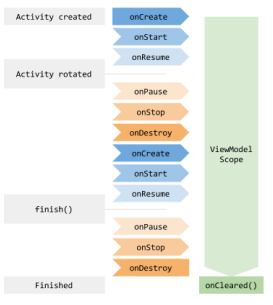
\includegraphics[scale=1]{Bilder/Viewmodel.PNG}

\subsection{MVVM im Eigenbau – Version 3}
\begin{minted}{Java}
public class UserActivity extends AppCompatActivity {
    private ActivityUserBinding binding;
    @Override
    protected void onCreate(Bundle savedInstanceState) {
        super.onCreate(savedInstanceState);
        User user = new User("Thomas", "Kälin", 36);
        UserViewModelFactory factory = new Use...Factory(user);
        UserViewModel viewModel = new ViewModelProvider(
        this, factory).get(UserViewModel.class);
        binding = ActivityUserBinding.inflate(...);
        binding.setVm(viewModel);
        binding.setLifecycleOwner(this);
        setContentView(binding.getRoot());
    }
}
public class UserViewModel extends ViewModel {
// Rest wie zuvor
}
public class UserViewModelFactory
            implements ViewModelProvider.Factory {
    private final User user;
    public UserViewModelFactory(User user) {
        this.user = user;
    }
    @Override
    public <T extends ViewModel> T create(Class<T> class) {
        return (T) new UserViewModel(user);
    }
}
\end{minted}
Lifecycle-Aware-Components reagieren auf Änderungen. Zustandslogik verschiebt sich vom Owner zum Observer. 

Interaktion zwischen Fragemnts kann sehr komplex werden (viele Callbacks). ViewModels können helfen aber Fragments verlieren die Unabhängigkeit.

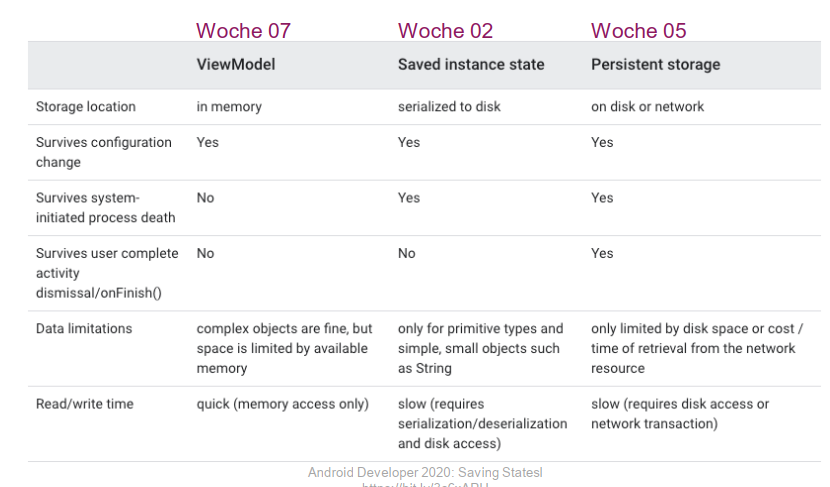
\includegraphics[scale=0.5]{Bilder/StorageLocationt.PNG}
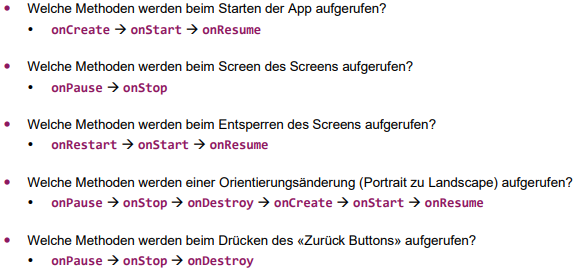
\includegraphics[scale=0.45]{Bilder/welcheMethodenAktion.png}

\section{Übungen}
«Schriftgrösse» nur einfluss auf sp\\
Starten einer Acitvity, welche nicht existiert, wirft eine Exception
\begin{minted}{Java}
Button browserButton = findViewById(R.id.buttonBrowser);
browserButton.setOnClickListener(v -> {
    Intent intent = new Intent(Intent.ACTION_VIEW,
                    Uri.parse("http://www.ost.ch"));
    if (intent.resolveActivity(getPackageManager()) != null) {
        startActivity(intent);
    }
});
\end{minted}
Wenn onClick Events im XML deklariert werden, werden die zur Laufzeit via Reflection auf eine gleichnamige Methode gemappt. Führt zu Exceptions zur Laufzeit bei falschem Namen.

\begin{minted}{Java}
final Runnable updateUi = new Runnable() {
// wie gehabt
};
Runnable background = new Runnable() {
@Override
public void run() {
    Thread.sleep(3000);
    Looper looper = Looper.getMainLooper();
    Handler handler = new Handler(looper);
    handler.post(updateUi);
}};
Thread thread = new Thread(background);
thread.start();
\end{minted}
\end{multicols*}
\end{document}